\section{Introduction}\label{sec:intro}

WebAssembly, commonly referred to as Wasm, is a versatile and efficient binary
instruction format that enables high-performance execution of code across
diverse environments, from web browsers to edge devices. The design philosophy
of WebAssembly revolves around platform independence, security, and efficient
performance, resulting in a versatile technology that bridges the gap between
high-level programming languages and the web ecosystem. As the adoption of WebAssembly
gains momentum, a continuous stream of new features is incorporated, extending
the capabilities of the language.

At the heart of WebAssembly's functionality lies its execution semantics, which
define how WebAssembly programs operate. The behavior of a WebAssembly program
is defined in terms of an abstract machine that models the program's state.
This abstract machine encompasses a stack to record operand values and control
constructs, as well as an abstract store housing global state information. The
execution process unfolds by iteratively executing each instruction of the
WebAssembly program, one step at a time. Each step alters the internal state of
the abstract machine, with the precise effects being specified by reduction
rules within the operational semantics.

The official WebAssembly specification~\cite{wasmspec} meticulously documents
the execution semantics using the LaTeX framework, presenting them in two
complementary yet equivalent forms: prose and formal notation. Prose notation
provides a stepwise, algorithmic description of WebAssembly's execution
semantics, offering explicit guidance on the operations to be executed on
various parts of the program state and their sequential order. This prose
notation aims to provide a human-readable understanding of how WebAssembly
instructions operate.  In contrast, formal notation articulates these semantics
through mathematical, declarative rules. This formal representation closely
resembles the original operational semantics, comprising reduction rules that
correspond to each WebAssembly instruction. The dual representation serves to
cater to comprehension of both language implementers and designers, ensuring
clarity and correctness within the language specification.

\begin{figure}
  \centering
  \begin{subfigure}[b]{0.45\textwidth}
    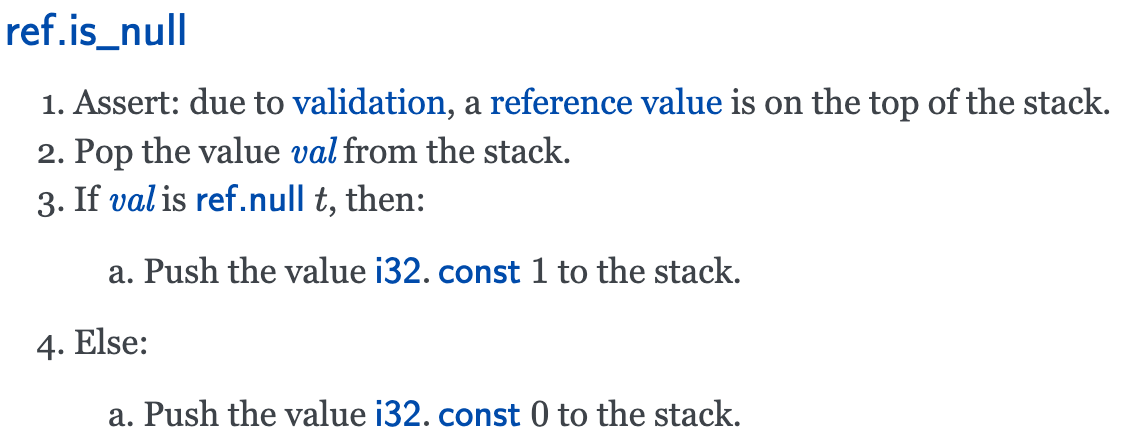
\includegraphics[width=\textwidth]{img/prosespec1}
    \caption{Prose notation}
    \label{fig:prosespec1}
  \end{subfigure}
  \hfill
  \begin{subfigure}[b]{0.45\textwidth}
    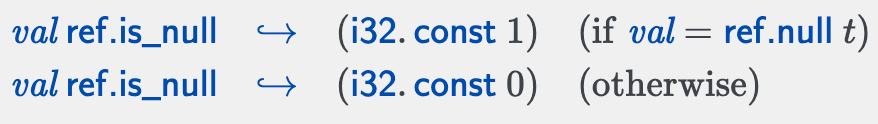
\includegraphics[width=\textwidth]{img/formalspec1}
    \caption{Formal notation}
    \label{fig:formalspec1}
  \end{subfigure}
  \begin{subfigure}[b]{0.45\textwidth}
    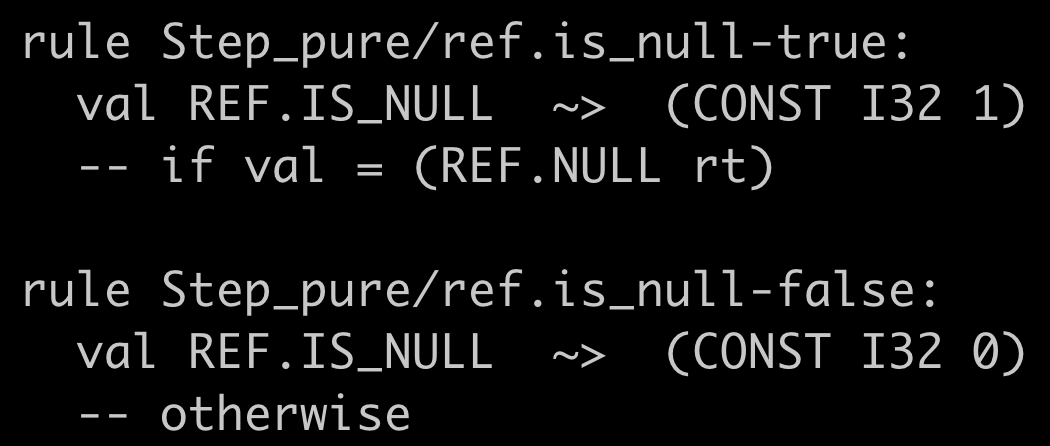
\includegraphics[width=\textwidth]{img/dsl1}
    \caption{DSL}
    \label{fig:dsl1}
  \end{subfigure}

  \caption{Semantics of `ref.is\_null`}
  \label{fig:spec1}
\end{figure}

In Figure~\ref{fig:spec1}, we present an illustration of how the specification
defines the execution semantics of the `ref.is\_null` WebAssembly instruction.
This instruction evaluates whether a given WebAssembly value is null. In
Figure~\ref{fig:prosespec1}, we specify its behavior using prose notation. The
description begins by asserting the existence of a value with a type of
`reference` at the top of the stack in line 1. Subsequently, in line 2, the
value is removed from the stack.  Depending on whether the removed value is
`ref.null t` or not, either the integer value 1 or 0 is pushed onto the stack
in lines 3-a or 4-a, respectively. In Figure~\ref{fig:formalspec1}, we provide
the operational semantics using formal notation, using two reduction rules. The reduction rule specifies
the shape of the stack before and after executing one step, potentially with
side conditions indicating when this reduction should occur. For instance, the
stack `val ref.is\_null` should reduce to (i32.const 1) only if `val` equals
`ref.null t`, and otherwise, it should reduce to (i32.const 0).

%Creating and maintaining this meticulous specification holds paramount
%significance as it forms the foundation for consistent and reliable behavior
%among WebAssembly programs across different implementations. This is crucial
%because developers, implementers, and tool creators need a comprehensive
%understanding of these semantics. This understanding is essential for building
%WebAssembly implementations that are not only robust but also optimized for
%efficiency, with the specification playing a pivotal role in facilitating this
%understanding. The ongoing evolution and growing adoption of WebAssembly
%further emphasize the heightened importance of precision and clarity within
%this documentation. As the WebAssembly ecosystem continues to develop and
%establish its presence, the accuracy and clarity of the specification become
%even more critical to ensure smooth integration and dependable execution.

The challenge of manually crafting and maintaining precise specifications is
particularly daunting due to the intricate nature of the documentation process.
Compounded by the utilization of the complex LaTeX typesetting system, the
manual authorship of these specifications becomes a laborious and error-prone
endeavor. It demands meticulous attention to detail for accurate
representation, making it susceptible to various errors, typos, or
inconsistency within specification. A case in point is the incorporation of 5
proposals for new features into Wasm 2.0. A substantial number of new
instructions, including a staggering 80 SIMD instructions, were added,
necessitating the manual composition of both formal and prose specifications
for each instruction. Moreover, the specifications of several existing
instructions underwent modifications. In the midst of this process, several
errors found its way into the specification of new or modified instructions,
one of which took two years to be rectified. This example, exemplified by the
expansion to Wasm 2.0, underscores the challenges posed by manually crafting and
maintaining the specification, demanding a labor-intensive process and
entailing the risk of errors. Given WebAssembly's planned extensions beyond 3.0,
driven by over 25 proposals, addressing this challenge becomes increasingly
critical.

In response to the challenges of crafting precise specifications manually, the
Wasm community has introduced a promising solution in the form of $\dsl$
(WebAssembly Domain Specific Language). It is a domain-specific language
tailored to describing the standard of WebAssembly, including its execution
semantics. $\dsl$ serves as the single source of truth for the WebAssembly semantics.
Once the operation semantics of WebAssembly is articulated using this
specialized language, numerous other 'representations' of the semantics can be
automatically generated, including interpreters, test suites, mechanized
proofs, and notably, the specification document.  By translating $\dsl$ as
front-end into LaTeX for both formal and prose specification as back-ends,
documenting the specification becomes a more streamlined process, potentially
reducing the burden of manual specification writing.  Moreover, this systematic
translation provides much higher confidence in the trustworthiness of the
generated specification compared to a manually generated one.

The key advantage of $\dsl$ lies in its ability to offer a clear, visually
aligned representation of the operational semantics of WebAssembly that is easy
to read and write. Figure~\ref{fig:dsl1} illustrates the semantics of
`ref.is\_null`, described using $\dsl$. Just like the operational semantics,
each reduction rule contains the left-hand side and right-hand side notating
the stack of the abstract machine before and after the reduction, and premises
denoting the condition for that reduction to happen.

Generating a formal notation specification from $\dsl$ is relatively
straightforward, thanks to this design. Since both $\dsl$ and formal
specifications adopt a declarative approach based on mathematical reduction
rules, the translation from $\dsl$ to formal notation can be achieved through a
single, linear scan of the $\dsl$. This one-to-one correspondence minimizes the
risk of generating a specification that deviates from the intended execution
semantics outlined in $\dsl$. Even in cases where discrepancies arise, they can
be readily identified and rectified.

Generating prose notation specification, however, presents a distinct and
intricate challenge. In contrast to $\dsl$, prose notation entails an
algorithmic, step-by-step description of execution semantics. The translation
between these two styles is not straightforward, as it necessitates the mapping
of declarative statements to algorithmic prose while ensuring consistency with
the formal specification.

\begin{figure}
  \centering
  \begin{subfigure}[b]{0.45\textwidth}
    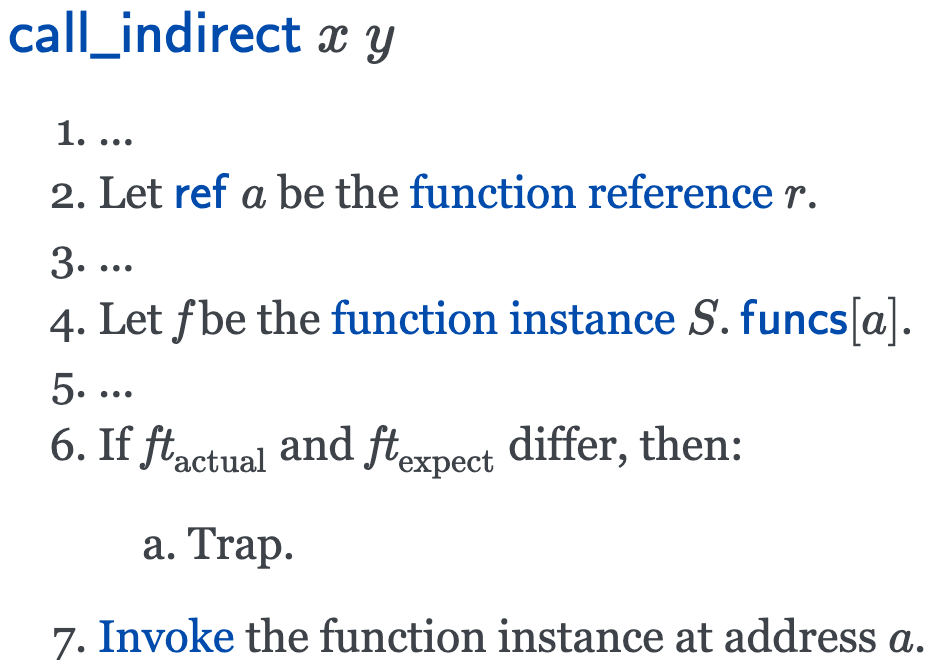
\includegraphics[width=\textwidth]{img/prosespec2}
    \caption{Prose notation}
    \label{fig:prosespec2}
  \end{subfigure}
  \hfill
  \begin{subfigure}[b]{0.45\textwidth}
    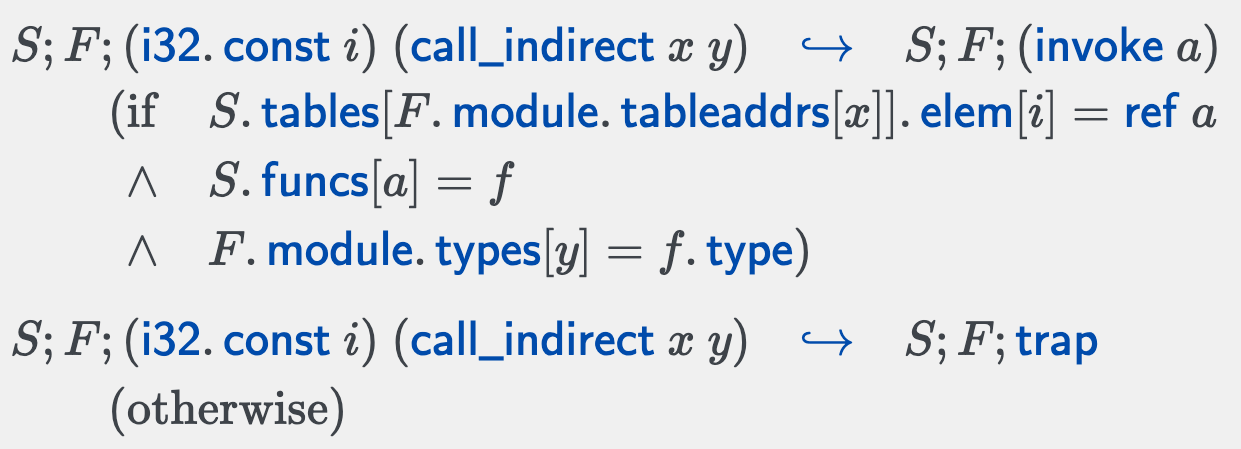
\includegraphics[width=\textwidth]{img/formalspec2}
    \caption{Formal notation}
    \label{fig:formalspec2}
  \end{subfigure}

  \caption{Semantics of `call\_indirect`}
  \label{fig:spec2}
\end{figure}

Figure~\ref{fig:spec2} illustrates one of these challenges, depicting the
manually-written specifications of the WebAssembly `indirect\_call` instruction. In
the formal specification (Figure~\ref{fig:formalspec2}), three premises are
presented, each comprising a simple equality. These premises are translated
into three instructions on line 2, 4, and 6 in the prose specification
(Figure~\ref{fig:prosespec2}), respectively. Notably, despite their identical
format of simple equality, some of these equalities are intended to establish a
new variable, while others are designed to serve as conditions. Consequently,
the first two are translated into the `Let` statement, as seen in lines 2 and 4,
while the last premise is transformed into the `If` statement in line 6. Adding
to the complexity, the three premises in the formal specification could be
arranged in any order, but the translated statements must adhere to a specific
fixed order due to interdependencies. This problem of inferring the role and
order of the premises, which we refer to as "animation," has been shown to be
NP-hard.

Furthermore, the inherent disparity between prose and formal notations poses a
challenge in ensuring that the generated prose accurately reflects the intended
behavior of the formal semantics. As an illustration, the prose specification
in Figure~\ref{fig:prosespec2} introduces temporary variables, such as
ft\_actual or ft\_expect, which were absent in the formal specifications
presented in Figure~\ref{fig:formalspec2}. This divergence complicates manual
verification of consistency since one must meticulously track such deviations.
Given that the process of prose generation is notably susceptible to errors due
to its intricate translation nature, the pursuit of a methodology to
systematically verify its alignment with the formal notation stands as a
substantial research endeavor.

In response to these challenges, we propose a novel solution: Algorithmic
Language ($\al$), an executable language that closely resembles the structure
and style of prose notation. Our approach seeks to automate and enhance the
process of generating prose descriptions from the formal semantics described in
$\dsl$. We achieve this in two pivotal steps. First, we establish an automated
pipeline for the translation of $\dsl$ into $\al$. Subsequently, we generate
prose descriptions by stringifying the translated $\al$. We also identify the
challenges encountered during the process including the animation problem
previously mentioned, and suggest the effective, lightweight solutions for
them. Furthermore, to underscore the correctness and reliability of the
generated prose, we have developed an interpreter for $\al$ which enables
automatic and rigorous testing of the behavior described by the translated
$\al$ against the official WebAssembly test suite. Our results confirm the
consistency and accuracy of our methodology, boasting a 100\% pass rate across
official WebAssembly tests, thereby validating the fidelity of the generated
prose descriptions.

In summary, this paper offers the following key contributions:

\begin{itemize}
\item We provide a formal definition of the syntax and semantics of
Algorithmic Language ($\al$), an executable language designed to resemble prose
specification.
\item We present an automated method for generating prose specification from
the execution semantics of WebAssembly described in $\dsl$, and provide the solutions for
the identified challenges during the process.
\item We establish the correctness and reliability of our automatically
generated prose descriptions by subjecting them to comprehensive testing
against the official WebAssembly test suite.
\end{itemize}

The subsequent sections of this paper will delve into the specifics of our
methodology, detailing the creation of $\al$, the translation process from
$\dsl$ into $\al$ and the identified challenges, the development of the $\al$
interpreter, and the comprehensive testing framework employed. Through this
exploration, we aim to not only address the challenges associated with prose
notation in WebAssembly, but also explore the potential of $\al$ as a transformative
tool for enhancing the accuracy and efficiency of programming language
specifications in general.
